\subsection{Test Introduction}
Given we are working in a \emph{mesh} network in which nodes may join
and leave frequently and without coordination an interesting problem
is how the routing protocol handles the sudden loss of one of its
routes. From the point of view of a user the most important factor in
this scenario is the time window in which he is cut off from the
network.

This is rationale behind the following test in which we measured the
convergence time of \batman\ and \olsr\ when subjected to a forced
link removal.

\subsection{Topology}
 The topology of the network is the one depicted in
Picture~\ref{pic:LayoutConvergence} . The laptops are disposed in a
diamond shaped topology with the \emph{source} and \emph{sink} nodes
at the boundaries. The node 10.0.0.66 is the \emph{preferred} path
from the \emph{source} to the \emph{sink}.

\Picture{images/convergence}
        {.90\columnwidth}
        {Configuration with single direct link}
        {pic:LayoutConvergence}

The \emph{iptables} configuration we use to setup such a topology is
the following:

\begin{itemize}
\item On 10.0.0.65 (source):

\begin{verbatim}
iptables -A INPUT -m mac --mac-source $(sinkMAC) -j DROP;
\end{verbatim}

\item On 10.0.0.66 (preferred)
\begin{verbatim}
iptables -A INPUT -m mac --mac-source $(preferredMAC) -j DROP;
\end{verbatim}

\item On 10.0.0.68 (secondary)
\begin{verbatim}
iptables -A INPUT -m mac --mac-source $(secondaryMAC) -j DROP;
\end{verbatim}

\item On 10.0.0.67 (sink)
\begin{verbatim}
iptables -A INPUT -m mac --mac-source $(sourceMAC) -j DROP;
\end{verbatim}
\end{itemize}

\subsection{Test structure}
A single iteration of the experiment consists in the following phases:
\begin{enumerate}
\item second 0: start experiment
\item second 10: start \netperf\ measurement
\item second 40: 10.0.0.66 network interface shutdown
\item second 70: test end
\end{enumerate}

We used the result of \netperf\ to measure the time window in
which the \emph{source} was't able to communicate with the
\emph{sink}. We could have simplified our lives by just using ping to
collect this information, but we wanted to also give some indication
on the throughput before and after the route changed. As it turned out
however, \netperf\ is not the most stable software: most of the times
it cold not resume the packet flow after the route change happened (even if
ping worked fine). To circumvent this problem we let \netperf\ perform
an alternative kind of test which measured the number of transaction
per second (with a transaction being characterized as an exchange of a
single request and a single response).
We then combined this information with the data gathered
by \emph{Wireshark} and the log of the routing protocol to extrapolate
the instant in which the route was actually changed.

A problem we had to face was how to force node 10.0.0.66 to be the
preferred route. In \olsr\ we exploited a configuration parameter
which let us penalize (in this case by a factor of 0.5) the alternate
route by hand:

\begin{verbatim}
LinkQualityMult 10.0.0.68 0.8
\end{verbatim}

\batman\ however proved itself more problematic. After a long search
we were unable to find any \emph{clean} way of dealing with this
matter. We then decided to address the problem from another angle.
At first we thought about using an \emph{iptables} rulo to impose a
limit on the number of packet allowed to be sent by the node
10.0.0.68. This choice however didn't satisfy us as it might have had
repercussions on the result of our test which we weren't able to
foreseen.

In the end we exploit our understanding of the protocol to \emph{game
  it}: we started the \batman\ daemon on node 10.0.0.68 with 5 seconds
delay. Thanks to the sliding window mechanism described in section
\ref{bla} and the limited duration of our experiment we were certain
that the preferred route would be through node 10.0.0.66. In case
there was any doubt about our reasoning, this consideration is
sustained both by the protocol log and the \emph{Wireshark}
recordings.


\subsection{\batman}
In this section we present the result we obtained for
\batman. Picture~\ref{pic:batman_convergence} show a summary of the
entire test whereas Picture~\ref{pic:batman_convergence_time}
and~\ref{pic:batman_convergence_change} show the respectively the
details of the convergence time and the route change instant.
Finally all the relative statistics are reported in
Table~\ref{tab:convergence_batman}.

The 3 dashed lines represent, from left to right, the start of the
\netperf\ measurement, the forced removal of node 10.0.0.66 and the
mean convergence time. The red dots indicate all the single
transaction per second data point. Finally the horizontal line shows
the route used by the source (where green corresponds to 10.0.0.66 and
blue to 10.0.0.68).

  \Picture{images/convergence_batman_plot}
               {\textwidth}
               {Convergence plot while using \batman\ as routing protocol}
               {pic:batman_convergence}


\begin{figure}[bhtp]
  \begin{minipage}[b]{0.5\linewidth}
    \centering
    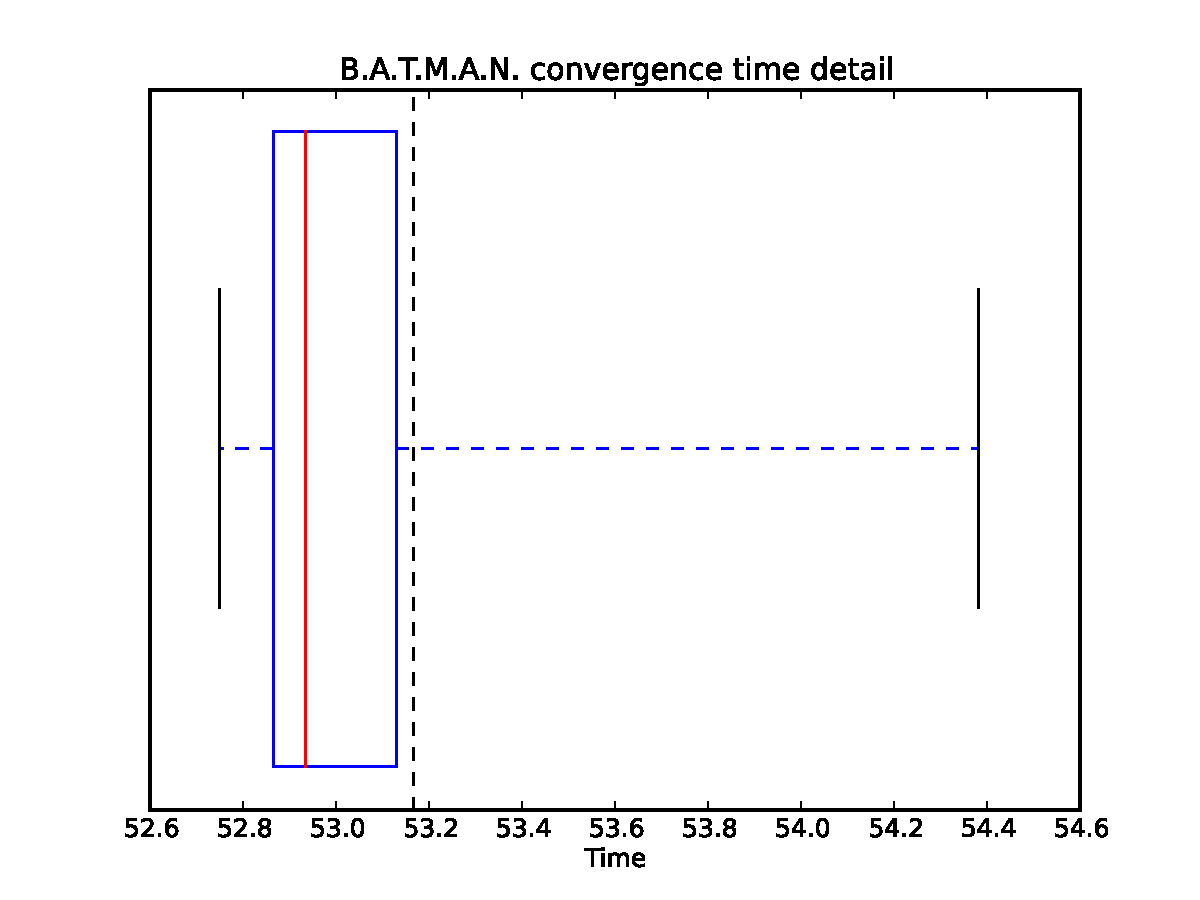
\includegraphics[width=\linewidth]{images/convergence_batman_plot_convergence_time}
    \caption{Detail of the convergence instant while using \batman\ as routing protocol}
    \label{pic:batman_convergence_time}
  \end{minipage}
  \hspace{0.5cm}
  \begin{minipage}[b]{0.5\linewidth}
    \centering
    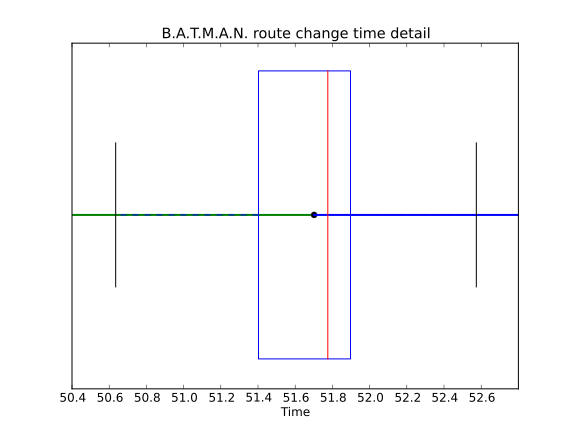
\includegraphics[width=\linewidth]{images/convergence_batman_plot_nexthop_change}
    \caption{Detail of the instant in which \batman\ changed the
                 preferred route}
    \label{pic:batman_convergence_change}
  \end{minipage}
\end{figure}


       \begin{table}[htbp]
            \centering
            \begin{tabular}{rccccccc}
            \toprule
            Kind & Average & Variance & Min & 1st Quartile &
            Median & 3rd Quartile & Max \\
            & \footnotesize{sec} & & \footnotesize{sec} & \footnotesize{sec} &
            \footnotesize{sec} & \footnotesize{sec} & \footnotesize{sec} \\
            \midrule
            Convergence & 13.166  & 0.250 & 12.749 & 12.856 & 12.935 & 13.149 &14.383\\
            Route change & 11.655 & 0.234 & 10.635 & 11.317 & 11.775 & 11.926 & 12.574\\
            \bottomrule
            \end{tabular}
            \caption{Statistics on the convergence anche route change
              instants of \batman.}
            \label{tab:convergence_batman}
        \end{table}

\clearpage
\subsection{\olsr}
In this section are included the result for \olsr.
In Picture~\ref{pic:olsr_convergence} is shown the summary of our
test. A zoomed view of the convergence instant and next-hop change
instant is reported respectively in
Picture~\ref{pic:olsr_convergence_time} and~\ref{pic:olsr_convergence_change}.

  \Picture{images/convergence_olsr_plot}
               {\textwidth}
               {Convergence plot while using \olsr\ as routing protocol}
               {pic:olsr_convergence}

\begin{figure}[bhtp]
  \begin{minipage}[b]{0.5\linewidth}
    \centering
    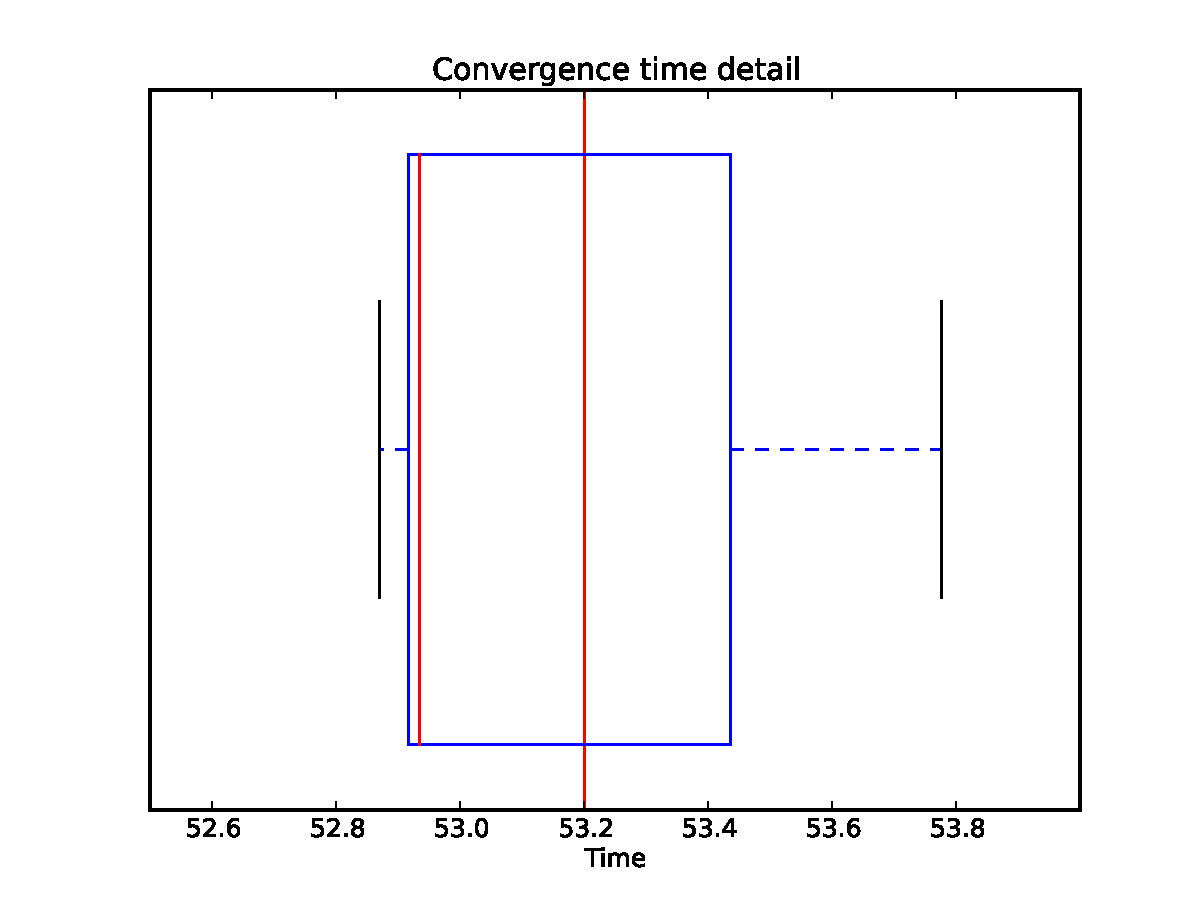
\includegraphics[width=\linewidth]{images/convergence_olsr_plot_convergence_time}
    \caption{Detail of the convergence instant while using \olsr\ as routing protocol}
    \label{pic:olsr_convergence_time}
  \end{minipage}
  \hspace{0.5cm}
  \begin{minipage}[b]{0.5\linewidth}
    \centering
    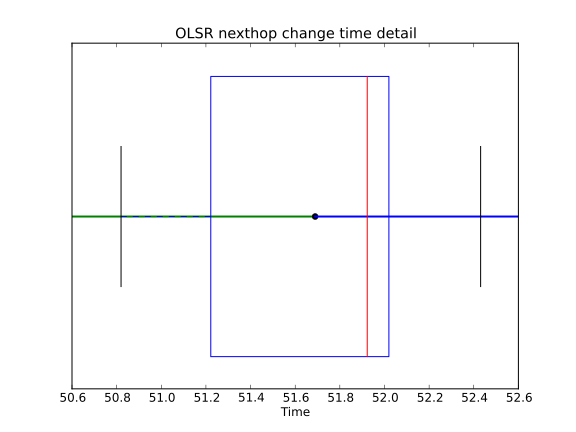
\includegraphics[width=\linewidth]{images/convergence_olsr_plot_nexthop_change}
    \caption{Detail of the instant in which \olsr\ changed the
                 preferred route}
    \label{pic:olsr_convergence_change}
  \end{minipage}
\end{figure}

       \begin{table}[htbp]
            \centering
            \begin{tabular}{rccccccc}
            \toprule
            Kind & Average & Variance & Min & 1st Quartile &
            Median & 3rd Quartile & Max \\
            & \footnotesize{sec} & & \footnotesize{sec} & \footnotesize{sec} &
            \footnotesize{sec} & \footnotesize{sec} & \footnotesize{sec} \\
            \midrule
            Convergence & 13.201 & 0.118 & 12.870 & 12.916 & 12.935 & 13.560 &13.776 \\
            Route change & 11.460 & 0.262 & 10.627 & 11.028 & 11.131 &11.827 & 12.238 \\
            \bottomrule
            \end{tabular}
           \caption{Statistics on the convergence anche route change
              instants of \olsr.}
            \label{tab:convergence_olsr}
        \end{table}
